\documentclass{standalone}

\begin{document}


\documentclass{standalone}

\begin{document}

\chapter[Deep Learning]{Deep Learning - Neural Network algorithms}\label{chapter2:neural}

Description of the modern deep neural networks.
Computational problems and potential applications

\end{document}
 % Neural Network introduction

\documentclass{standalone}

\begin{document}

\section[Fully Connected Neural Network]{Fully Connected Neural Network}\label{NN:connected}

To overcome problems arising from the Simple Perceptron model we can join together multiple Perceptron units into a more complex network of interaction in which the output of a neuron feed-forward the input of the next one.
This is the Multi-layers Perceptron (MLP) configuration and if the graph is fully connected, i.e each neuron is connected to all the others, we talk about \emph{fully connected neural networks} (or \emph{dense} neural network, DNN).

Given the Perceptron formulas, the extrapolation to the MLP architecture is straight-forward and given by

$$
y = \sigma\left(X \cdot W + W_0 \right)
$$
\\
where we simply pass from the vector formulation to the matrix one.
The updating rule consequentially becomes

$$
\delta W = \delta W + X^T \cdot \left( \frac{\partial f(y)}{\partial y} \cdot \delta^l \right)  \quad\quad \delta W_0 = \sum_{i=0}^{m}\frac{\partial f(y)}{\partial y_i} \cdot \delta_i^l
$$
\\
where also in this case we simply pass to the matrix formalism and we convert the discrete format to a continuous one, i.e with continuous values we convert the error to a partial derivative.
In the above equation $\delta^l$ represents the error pass from the next layer in the network structure\footnote{
  In the Back-Propagation Algorithm the error is passed by each layer to the previous one, starting from the output error computed according to chosen loss function.
}.

From the re-iteration of such structures we can join together multiple fully connected layers and so obtain multiple neuron layers jointly together with different levels of complexity and units (an input layer followed by multiple \emph{hidden} layers).

The fully connected Neural Networks overcome the told above \emph{Perceptron} problems using a combination of linear functions (single \emph{Perceptron} units) and they gain more useful properties:

\begin{itemize}

\item If the activation functions of \emph{all} the hidden units in the Neural Network are linear, then the network architecture is equivalent to a network without hidden units.

\item If the number of hidden units is smaller than either the number of input units either the number of output ones, then the network can generate transformations from inputs to outputs as much general as possible since the information is lost in the dimensionality reduction performed by the hidden units.

\item We can find multiple weight configurations, i.e $W$ matrices, which give us the same mapping function from inputs to outputs.

\end{itemize}


\end{document}

\documentclass{standalone}

\begin{document}


\subsubsection[Matrix Product]{Matrix Product}\label{NN:gemm}

Despite the mathematical formulation of the model we have to take into account also an efficient implementation.
From a numerical point-of-view we can notice that all the computation required by this kind of Networks (or layer if we consider it into an hybrid Neural Network architecture as we will see in the next sections) can be summarized into the matrix product evaluation.
The matrix product is a well-known numerical problem and its algorithmic complexity can be hardly reduced under $O(N^3)$\footnote{
  The complexity is often given in the assumption of only square matrices $(N\times N)$ involved in the computation.
  For no-square matrix the algorithm complexity is given by the product of the three possible different matrix dimensions involved ($(N\times K) = (N\times M)(M\times K)$ brings to $O(NMK)$ complexity).
  More sophisticated implementation of the algorithm are able to reduce the algorithm complexity (e.g Strassen algorithm) but neither implementation is able to overcome the $O(N^{2.7})$ complexity up-to-now.
}.
A crucial role on this kind of algorithms is played by the cache accesses.
The CPU cache is the hardware cache used by the CPU to store small portion of data in order to reduce the average cost (in time or energy consumption) to data access from the main memory.
Cache optimization is one of the most difficult parts to perform writing an algorithm, but it leads to highest performance gains.

In the matrix product we have to multiply each row of a matrix $A$ by each column of a second matrix $B$.
We work in the assumption that each matrix is stored into an array of 1D or 2D without nested structures.
In this case we can access to a contiguous memory portion of the first matrix since each row is given by a series of sequential index locations (the row elements are given by $x[0], x[1], \dots, x[N]$).
This configuration allows the cache optimization in the access to the first matrix, since we can store in a small portion of cache memory a series of row elements and use them in a vectorization environment.

From the second matrix we have to extract the elements from each column.
This means that the elements are given by a discontinuous portion of memories (the column elements are given by $x[0], x[M], x[2M], \dots, x[N(M-1)]$).
In this case we can not insert a full column into the cache memory and in consequence we have a \emph{cache-miss} at each iteration\footnote{
  The \emph{cache-miss} happens when a required data can not be found into the cache and so its search has to be done in the main memory (RAM).
}.

The simple matrix product as given by row-column multiplication is already affected by an intrinsic numerical problem which can drastically affect its performances.
The simplest workaround of this issue is to perform a transposition of the second matrix to obtain a row-row matrix product\footnote{
  In the discussion we have silently ignored the problems of matrix storage and the cache optimization for the resulting matrix accesses but in the above discussion we want to focus only on the main problems raising from the matrix product.
}.
In this way both matrices can be accessed in a sequential order.
The total complexity of the computation increase to $O(N^2)$ (for the matrix transposition, in the better case) $+ O(N^3)$ (for matrix product) but the numerical performances increase due to the cache-miss minimization\footnote{
  The cache memory is a very tight portion of memory and it is impossible to completely remove cache-misses.
}.

Following back to our Neural Network implementation we can obtain the output values using the above technique.
Moreover, we can assume from the beginning that the transposition of weight matrix and so remove the $O(N^2)$ calculus from the matrix product.
This simple (but carefully studied) optimization allows to obtain better results in the feed-forward evaluation, but it paybacks a revision of the standard mathematical formulation and a carefully implementation of the code.

\begin{figure}[htbp]
\includegraphics[width=0.45\textwidth]{GEMM_schema.png}
\quad
\centering
\def\svgwidth{0.45\textwidth}
\documentclass{standalone}

\begin{document}


\subsubsection[Matrix Product]{Matrix Product}\label{NN:gemm}

Despite the mathematical formulation of the model we have to take into account also an efficient implementation.
From a numerical point-of-view we can notice that all the computation required by this kind of Networks (or layer if we consider it into an hybrid Neural Network architecture as we will see in the next sections) can be summarized into the matrix product evaluation.
The matrix product is a well-known numerical problem and its algorithmic complexity can be hardly reduced under $O(N^3)$\footnote{
  The complexity is often given in the assumption of only square matrices $(N\times N)$ involved in the computation.
  For no-square matrix the algorithm complexity is given by the product of the three possible different matrix dimensions involved ($(N\times K) = (N\times M)(M\times K)$ brings to $O(NMK)$ complexity).
  More sophisticated implementation of the algorithm are able to reduce the algorithm complexity (e.g Strassen algorithm) but neither implementation is able to overcome the $O(N^{2.7})$ complexity up-to-now.
}.
A crucial role on this kind of algorithms is played by the cache accesses.
The CPU cache is the hardware cache used by the CPU to store small portion of data in order to reduce the average cost (in time or energy consumption) to data access from the main memory.
Cache optimization is one of the most difficult parts to perform writing an algorithm, but it leads to highest performance gains.

In the matrix product we have to multiply each row of a matrix $A$ by each column of a second matrix $B$.
We work in the assumption that each matrix is stored into an array of 1D or 2D without nested structures.
In this case we can access to a contiguous memory portion of the first matrix since each row is given by a series of sequential index locations (the row elements are given by $x[0], x[1], \dots, x[N]$).
This configuration allows the cache optimization in the access to the first matrix, since we can store in a small portion of cache memory a series of row elements and use them in a vectorization environment.

From the second matrix we have to extract the elements from each column.
This means that the elements are given by a discontinuous portion of memories (the column elements are given by $x[0], x[M], x[2M], \dots, x[N(M-1)]$).
In this case we can not insert a full column into the cache memory and in consequence we have a \emph{cache-miss} at each iteration\footnote{
  The \emph{cache-miss} happens when a required data can not be found into the cache and so its search has to be done in the main memory (RAM).
}.

The simple matrix product as given by row-column multiplication is already affected by an intrinsic numerical problem which can drastically affect its performances.
The simplest workaround of this issue is to perform a transposition of the second matrix to obtain a row-row matrix product\footnote{
  In the discussion we have silently ignored the problems of matrix storage and the cache optimization for the resulting matrix accesses but in the above discussion we want to focus only on the main problems raising from the matrix product.
}.
In this way both matrices can be accessed in a sequential order.
The total complexity of the computation increase to $O(N^2)$ (for the matrix transposition, in the better case) $+ O(N^3)$ (for matrix product) but the numerical performances increase due to the cache-miss minimization\footnote{
  The cache memory is a very tight portion of memory and it is impossible to completely remove cache-misses.
}.

Following back to our Neural Network implementation we can obtain the output values using the above technique.
Moreover, we can assume from the beginning that the transposition of weight matrix and so remove the $O(N^2)$ calculus from the matrix product.
This simple (but carefully studied) optimization allows to obtain better results in the feed-forward evaluation, but it paybacks a revision of the standard mathematical formulation and a carefully implementation of the code.

\begin{figure}[htbp]
\includegraphics[width=0.45\textwidth]{GEMM_schema.png}
\quad
\centering
\def\svgwidth{0.45\textwidth}
\documentclass{standalone}

\begin{document}


\subsubsection[Matrix Product]{Matrix Product}\label{NN:gemm}

Despite the mathematical formulation of the model we have to take into account also an efficient implementation.
From a numerical point-of-view we can notice that all the computation required by this kind of Networks (or layer if we consider it into an hybrid Neural Network architecture as we will see in the next sections) can be summarized into the matrix product evaluation.
The matrix product is a well-known numerical problem and its algorithmic complexity can be hardly reduced under $O(N^3)$\footnote{
  The complexity is often given in the assumption of only square matrices $(N\times N)$ involved in the computation.
  For no-square matrix the algorithm complexity is given by the product of the three possible different matrix dimensions involved ($(N\times K) = (N\times M)(M\times K)$ brings to $O(NMK)$ complexity).
  More sophisticated implementation of the algorithm are able to reduce the algorithm complexity (e.g Strassen algorithm) but neither implementation is able to overcome the $O(N^{2.7})$ complexity up-to-now.
}.
A crucial role on this kind of algorithms is played by the cache accesses.
The CPU cache is the hardware cache used by the CPU to store small portion of data in order to reduce the average cost (in time or energy consumption) to data access from the main memory.
Cache optimization is one of the most difficult parts to perform writing an algorithm, but it leads to highest performance gains.

In the matrix product we have to multiply each row of a matrix $A$ by each column of a second matrix $B$.
We work in the assumption that each matrix is stored into an array of 1D or 2D without nested structures.
In this case we can access to a contiguous memory portion of the first matrix since each row is given by a series of sequential index locations (the row elements are given by $x[0], x[1], \dots, x[N]$).
This configuration allows the cache optimization in the access to the first matrix, since we can store in a small portion of cache memory a series of row elements and use them in a vectorization environment.

From the second matrix we have to extract the elements from each column.
This means that the elements are given by a discontinuous portion of memories (the column elements are given by $x[0], x[M], x[2M], \dots, x[N(M-1)]$).
In this case we can not insert a full column into the cache memory and in consequence we have a \emph{cache-miss} at each iteration\footnote{
  The \emph{cache-miss} happens when a required data can not be found into the cache and so its search has to be done in the main memory (RAM).
}.

The simple matrix product as given by row-column multiplication is already affected by an intrinsic numerical problem which can drastically affect its performances.
The simplest workaround of this issue is to perform a transposition of the second matrix to obtain a row-row matrix product\footnote{
  In the discussion we have silently ignored the problems of matrix storage and the cache optimization for the resulting matrix accesses but in the above discussion we want to focus only on the main problems raising from the matrix product.
}.
In this way both matrices can be accessed in a sequential order.
The total complexity of the computation increase to $O(N^2)$ (for the matrix transposition, in the better case) $+ O(N^3)$ (for matrix product) but the numerical performances increase due to the cache-miss minimization\footnote{
  The cache memory is a very tight portion of memory and it is impossible to completely remove cache-misses.
}.

Following back to our Neural Network implementation we can obtain the output values using the above technique.
Moreover, we can assume from the beginning that the transposition of weight matrix and so remove the $O(N^2)$ calculus from the matrix product.
This simple (but carefully studied) optimization allows to obtain better results in the feed-forward evaluation, but it paybacks a revision of the standard mathematical formulation and a carefully implementation of the code.

\begin{figure}[htbp]
\includegraphics[width=0.45\textwidth]{GEMM_schema.png}
\quad
\centering
\def\svgwidth{0.45\textwidth}
\input{./img/gemm.pdf_tex}
\caption{GEMM algorithms time performances.
\textsf{GEMM NN}: matrix multiplication considering both the matrices in \quotes{normal} format, i.e $A\cdot B$.
\textsf{GEMM NT}: matrix multiplication considering the first matrix in \quotes{normal} format and the second one transposed, i.e $A\cdot B^T$.
We perform 100 tests of 1K runs each of both the \textsf{GEMM} algorithms using the \textsf{einsum} function of \textsf{Numpy} library.
The values are rescaled according to the mean time of the \textsf{GEMM NN} algorithm.
}
\label{fig:gemm}
\end{figure}

In the proposed numerical implementations of this model we implement both the matrix product cases to compare the performance results.
We tested the two implementations inside \textsf{Python} using the \textsf{einsum} function provided by the \textsf{Numpy} package.
In particular, we evaluated the time-performances over 1000 applications of the two \textsf{GEMM} functions (\textsf{GEMM NN}, i.e considering both matrices with \quotes{normal} shapes; \textsf{GEMM NT}, i.e considering the first matrix as \quotes{normal} and the second transposed) considering matrices of shapes ($100\times100$).
We performed $500$ run and we saved the minimum time obtained over $10$ realizations.
In Fig.~\ref{fig:gemm} we show the results rescaled by the mean time (over the 500 realizations) of the \textsf{GEMM NN} algorithm (reference).
As can be seen in Fig.~\ref{fig:gemm} the speedup of the \textsf{GEMM NT} matrix is evident and it is always faster than \textsf{GEMM NN} algorithm with a maximum of $3.2$x in the speedup.

In the \textsf{Byron} library we provide a parallelized version of this algorithm with also an \textsf{avx} support.
In this way we could manually manage the register memory of the two matrices and obtain a faster \textsf{GEMM} algorithm (especially for dimensions proportional to powers of 2 which are very common in neural network models).

\end{document}

\caption{GEMM algorithms time performances.
\textsf{GEMM NN}: matrix multiplication considering both the matrices in \quotes{normal} format, i.e $A\cdot B$.
\textsf{GEMM NT}: matrix multiplication considering the first matrix in \quotes{normal} format and the second one transposed, i.e $A\cdot B^T$.
We perform 100 tests of 1K runs each of both the \textsf{GEMM} algorithms using the \textsf{einsum} function of \textsf{Numpy} library.
The values are rescaled according to the mean time of the \textsf{GEMM NN} algorithm.
}
\label{fig:gemm}
\end{figure}

In the proposed numerical implementations of this model we implement both the matrix product cases to compare the performance results.
We tested the two implementations inside \textsf{Python} using the \textsf{einsum} function provided by the \textsf{Numpy} package.
In particular, we evaluated the time-performances over 1000 applications of the two \textsf{GEMM} functions (\textsf{GEMM NN}, i.e considering both matrices with \quotes{normal} shapes; \textsf{GEMM NT}, i.e considering the first matrix as \quotes{normal} and the second transposed) considering matrices of shapes ($100\times100$).
We performed $500$ run and we saved the minimum time obtained over $10$ realizations.
In Fig.~\ref{fig:gemm} we show the results rescaled by the mean time (over the 500 realizations) of the \textsf{GEMM NN} algorithm (reference).
As can be seen in Fig.~\ref{fig:gemm} the speedup of the \textsf{GEMM NT} matrix is evident and it is always faster than \textsf{GEMM NN} algorithm with a maximum of $3.2$x in the speedup.

In the \textsf{Byron} library we provide a parallelized version of this algorithm with also an \textsf{avx} support.
In this way we could manually manage the register memory of the two matrices and obtain a faster \textsf{GEMM} algorithm (especially for dimensions proportional to powers of 2 which are very common in neural network models).

\end{document}

\caption{GEMM algorithms time performances.
\textsf{GEMM NN}: matrix multiplication considering both the matrices in \quotes{normal} format, i.e $A\cdot B$.
\textsf{GEMM NT}: matrix multiplication considering the first matrix in \quotes{normal} format and the second one transposed, i.e $A\cdot B^T$.
We perform 100 tests of 1K runs each of both the \textsf{GEMM} algorithms using the \textsf{einsum} function of \textsf{Numpy} library.
The values are rescaled according to the mean time of the \textsf{GEMM NN} algorithm.
}
\label{fig:gemm}
\end{figure}

In the proposed numerical implementations of this model we implement both the matrix product cases to compare the performance results.
We tested the two implementations inside \textsf{Python} using the \textsf{einsum} function provided by the \textsf{Numpy} package.
In particular, we evaluated the time-performances over 1000 applications of the two \textsf{GEMM} functions (\textsf{GEMM NN}, i.e considering both matrices with \quotes{normal} shapes; \textsf{GEMM NT}, i.e considering the first matrix as \quotes{normal} and the second transposed) considering matrices of shapes ($100\times100$).
We performed $500$ run and we saved the minimum time obtained over $10$ realizations.
In Fig.~\ref{fig:gemm} we show the results rescaled by the mean time (over the 500 realizations) of the \textsf{GEMM NN} algorithm (reference).
As can be seen in Fig.~\ref{fig:gemm} the speedup of the \textsf{GEMM NT} matrix is evident and it is always faster than \textsf{GEMM NN} algorithm with a maximum of $3.2$x in the speedup.

In the \textsf{Byron} library we provide a parallelized version of this algorithm with also an \textsf{avx} support.
In this way we could manually manage the register memory of the two matrices and obtain a faster \textsf{GEMM} algorithm (especially for dimensions proportional to powers of 2 which are very common in neural network models).

\end{document}


\input{./tex/Chapter2/NeuralNetwork/Activations.tex}
\documentclass{standalone}

\begin{document}


\subsection[Relu]{Rectified Linear Unit}\label{relu}

The ReLU (Rectified Linear Unit) activation functions are the most used into the modern Neural Networks models.
Their diffusion is imputed to their numerical efficiency and to the benefits they bring~\cite{}:

\begin{itemize}

\item Information disentangling: the main purpose of a Neural Network model is to tune a discriminant function able to associate a set of input to a prior-known output classes.
A dense information representation is considered \emph{entangled} because small differences in input highly modifies the data representation inside the network.
On the other hand, a sparse representation tends to guarantee a conservation of the learning features.

\item Information representation: different inputs can lead different quantities of useful informations.
The possibility to have null values in output (ref Tab.~\ref{tab:activations}) allows a better representation of the representation dimension inside the network.

\item Sparsity: sparsity representation of data are exponentially efficient in comparison to dense ones, where the exponential power is given by the number of no-null features~\cite{}.

\item Vanish gradient reduction: if the activation output is positive we have a no-bound gradient value.
%add other considerations

\end{itemize}

\end{document}


\documentclass{standalone}

\begin{document}

% https://victorzhou.com/blog/intro-to-cnns-part-1/
% https://towardsdatascience.com/a-comprehensive-guide-to-convolutional-neural-networks-the-eli5-way-3bd2b1164a53
% https://ujjwalkarn.me/2016/08/11/intuitive-explanation-convnets/

\subsection[Convolution function]{Convolution function}\label{NN:convolutional}

A big revolution into the Neural Network research field has been given by the introduction of convolution functions.
Convolutional Neural Network (CNN) are particularly designed for image analyses.
Convolution is the mathematical integration of two functions in which the second one is translated by a given value:

\begin{equation}
(f * g)(t) = \int_{-\infty}^{+\infty} f(\tau)g(t - \tau)d\tau
\end{equation}

In signal processing, this operation is also called \emph{crossing correlation} ad it is equivalent to the \emph{autocorrelation} function computed at a given point.
In image processing the first function is represented by the image $I$ and the second one is a kernel $k$ (or filter), which shifts along the image.
In this case we have a 2D discrete version of the formula given by:

\begin{equation}
\begin{aligned}
C = k * I
\\
C[i, j] = \sum_{u=-N}^{N} \sum_{v=-M}^{M} k[u, v] \cdot I[i - u, j - v]
\end{aligned}
\end{equation}
\\
where $C[i, j]$ is the pixel value of the resulting image and $N$, $M$ are the kernel dimensions.

The use of CNN in modern image analyses can be traced back to multiple causes.
First of all the image dimensions are increasingly bigger and thus the number of variables/features, i.e pixels, is often too big to manage with standard DNN\footnote{
  If we consider a simple image $224\times224$ with $3$ color channels we obtain a set of \numprint{150528} features.
  A classical DNN layer with this input size should have $1024$ nodes for a total of more than $150$ million weights to tune.
}.
Moreover, if we consider detection problems, i.e the problem of detecting a set of features (or an object) into a larger pattern, we want a system ables to recognize the object regardless of where it appears into the picture.
In other words, we want that our model would be independent by simple translations.

Both the above problems can be overcame by CNN models using a small kernel, i.e weight mask, which maps the full input.
A CNN is able to successfully capture the spatial and temporal dependencies in a signal through the application of relevant filters.

The main parameters of this function are given by the input dimensions and the filter/kernel dimensions, i.e the number of weights which we have to tune during the training.
This is the basic idea behind the convolution function, but in many cases (especially in modern deep learning Neural Networks) we can sophisticate it, playing with the possible movements of the filter mask.
In particular, aside the kernel mask-size, we can force the filter to jump along the image, i.e a discontinuous movement of the filter excluding some pixels.
This parameter, called \textsf{stride}, defines the number of pixels to jump and it is often used to further reduce the output dimensions.

Given this theoretical background we can implement the convolution function in many different ways, using different mathematical approaches: a study about the computational efficiency will tell us which is the best approach to choose.
The first (naive) approach is to use a brute force technique and implement the direct evaluation of the convolution function as described in the above equation.
This version is certainly the easier to implement, but its computational performances are so worst that, for sake of brevity, we excluded it from our tests\footnote{
  Compared to the other implementations the direct (brute force) convolution algorithm exceeds the computational time of order of magnitudes.
  For this reason it is not taken into account during our tests.
  A possible implementation in \textsf{C++} is however provided into the \href{https://github.com/Nico-Curti/Byron/blob/master/utility/winograd_test.cpp}{\textsf{Byron} library}.
}.

\begin{center}
\begin{figure}[htbp]
\centering
\includegraphics[width=0.85\textwidth]{im2col.png}
\caption{\textsf{im2col} algorithm scheme using a $2\times2$ filter on a image with 3 channels.
At the end of the \textsf{im2col} algorithm the \textsf{GEMM} is performed between weights and input image.
}
\label{fig:im2col}
\end{figure}
\end{center}

Taking into account what we have learned from the DNN models, we can re-formulate our problem using an efficient manipulation of the involved matrices to optimize the \textsf{GEMM} algorithm.
A direct convolution on an image of size ($W\times H\times C$), using a kernel mask of dimensions ($k \times k$), requires $O(WHCk^2)$ operations and thus several matrix products.
We can re-arrange the involved data to optimize this computation and evaluate a single matrix product: this re-arrangement is called \textsf{im2col} (or \textsf{im2row}) algorithm.
The algorithm is just a simple transformation which flats the original input into a bigger matrix, where each column carries all the elements which have to be multiplied for the filter mask into a single step\footnote{
  We work under the assumption that the weights matrix is already a flatten array and thus each row of the weights matrix represents the full mask.
}.
In this way we can immediately apply our \textsf{GEMM} algorithm on the full image.
In Fig.~\ref{fig:im2col} the main scheme of this algorithm is reported.
This algorithm optimizes the computational efficiency of the \textsf{GEMM} product but we have to store a lot of memory for the input re-organization in payback.

Using the mathematical theory behind the problem a third idea can arise using the well known Convolution Theorem: the Fourier transformation of our functions (that in this case are given by the input image and the weights kernel) can be reinterpreted into a simple matrix product in the frequency space.
This is certainly the most \quotes{physical} approach to solve this problem and probably the easier one since the Fourier Transformation is a well-known optimized algorithm, with several efficient implementations provided in literature.
One of the most efficient one is provided by the \textsf{FFTW} (\emph{Fast Fourier Transform in the West}) library~\cite{FFTW05}: \textsf{FFTW3} is an open source \textsf{Ansi-C} subroutine library for computing the Discrete Fourier Transform (DFT) in multiple dimensions, without constraints in input sizes or data types.
The library is not only computationally accurate, but it also provides an efficient parallel version for multi-threading applications.

A further implementation kind is given by linear algebra considerations (very closed to numerical considerations) and it is called \textsf{Coppersmith-Winograd algorithm}.
This algorithm was designed to optimize the matrix product and, in particular, to reduce the computational cost of its operations.
Suppose we have an input image given by just 4 elements and a filter mask with size equal to 3:

\begin{equation}
\mbox{img} = \left[\begin{array}{cccc} d0 & d1 & d2 & d3 \end{array}\right] \quad\quad \mbox{weights} = \left[\begin{array}{ccc} g0 & g1 & g2 \end{array}\right]
\end{equation}
\\
we can now use the \textsf{im2col} algorithm previously described and reshape our input image and weights into

\begin{equation}
\mbox{img} = \left[
\begin{array}{ccc}
d0 & d1 & d2 \\
d1 & d2 & d3
\end{array}
\right],
\quad\quad
\mbox{weights} = \left[
\begin{array}{c}
g0 \\
g1 \\
g2
\end{array}
\right]
\end{equation}
\\
given this data, we can simply compute the output as the matrix product of this two matrices.
The Winograd algorithm rewrites this computation as follow:

\begin{equation}
\mbox{output} = \left[
\begin{array}{ccc}
d0 & d1 & d2 \\
d1 & d2 & d3
\end{array}
\right]
\left[
\begin{array}{c}
g0 \\
g1 \\
g2
\end{array}
\right] = \left[
\begin{array}{c}
m1 + m2 + m3 \\
m2 - m3 - m4
\end{array}
\right]
\end{equation}
\\
where

\begin{equation}
\begin{aligned}
m1 = (d0 - d2)g0\quad\quad m2 = (d1 + d2)\frac{g0 + g1 + g2}{2}
\\
m4 = (d1 - d3)g2\quad\quad m3 = (d2 - d1)\frac{g0 - g1 + g2}{2}
\end{aligned}
\end{equation}
\\
where we can easily notice that the two fractions in $m2$ and $m3$ involve only weight quantities and thus they could be computed only one time for each filter (at each step).
Moreover, we have to manage $4$ \textsf{ADD} and $4$ \textsf{MUL} operations to calculate the $m_i$ quantities and $4$ other ADD to compute the result.
In doing normal matrix products we have to do $6$ \textsf{MUL} operations instead of $4$: the reduction of computational expensive \textsf{MUL} operations by a factor $1.5$x is very significant\footnote{
  A multiplication takes $7$ clock-cycles in a normal CPU while an add takes only $3$ clock-cycles.
}.
In this simple example we use a so-called $F(4, 3)$, i.e image of size $4$ and kernel of size $3$ which gives us $2$ convolutions.
More general formulations are $F(m\times m, r \times r)$ and if we use an image of size $4\times4$ and a kernel of size $3\times3$ we can compare the $16$ \textsf{MUL}s of the \textsf{Winograd} algorithm against the $36$ \textsf{MUL}s which are required by the normal matrix product ($2.25$x).
The \textsf{Winograd} efficiency has been widely proved for CNNs, especially when the kernel size is small.
In our \textsf{Byron} library we provide its implementation for kernel sizes equal to $3$, since the numerical generalization is not straightforward\footnote{
  We would also highlight that this formulation is valid only if we consider unitary strides.
}.

We tested the computational-time of each algorithm on different random images.
The tests were performed on a classical bioinformatics server (128~GB RAM memory and 2 CPU E5-2620, with 8 cores each) and we considered only kernel sizes equal to $3$ (\textsf{Winograd} constrain) varying input dimensions and number of filters.
In Fig.~\ref{fig:winograd_timing} we show the results of our simulations using the \textsf{im2col} values as reference\footnote{
  The \textsf{im2col} algorithm can be found in the major part of Neural Network library and it is also the only convolution function implemented in the \textsf{darknet} library, which is a reference for our work.
}.

\begin{figure}[htbp]
\centering
\def\svgwidth{0.8\textwidth}
\input{./img/winograd_timing.pdf_tex}
\caption{Time performances of different convolution algorithms: \textsf{im2col} (orange, reference), \textsf{FFTW3} (green, fast Fourier transformation using the \textsf{FFTW3} library) and \textsf{Winograd} (blue).
The values are normalized according to the \textsf{im2col} results since it is the most common convolution algorithm.
The tests were performed on different input sizes (width/height), keeping fixed the number of channels and the number of filters.
The tests were performed using a \textsf{C++} implementation of the three methods.
}
\label{fig:winograd_timing}
\end{figure}

In all our simulations we found a visible speedup using the \textsf{Winograd} algorithm against the other two algorithms: for small dimensions we obtained more than $5$x against the \textsf{im2col} and $25$x against the \textsf{fftw} implementation.
The worst algorithm is certainly the \textsf{fftw} one which, despite the efficient \textsf{FFTW3} parallel-library, is always more than $5$ times slower than the reference.
However, it is interesting notice how the \textsf{fftw} implementation is able to reach the best performances when the dimensions are proportional to powers of $2$, as expected from the mathematical theory behind the Discrete Fourier Transformation.

We can conclude that the \textsf{Winograd} algorithm is certainly the best choice when we have to perform a 2D convolution.
The payback of this method is given by the rigid constraints related to the mask sizes and strides: when it is possible it remains the best solution, but in all the other cases the \textsf{im2col} implementation is a relatively good alternative.
The efficiency of \textsf{Byron} library follows the efficiency of the \textsf{Winograd} algorithm, since the major part of layers in modern deep learning Neural Network models are Convolutional layers with sizes equal to $3$ and unitary strides.

%https://victorzhou.com/blog/intro-to-cnns-part-1/


\end{document}

\documentclass{standalone}

\begin{document}

\subsection[Pooling function]{Pooling function}\label{NN:pooling}

Output Neural Network feature maps often suffer of sensitivity about features location in the input.
One possible approach to overcome this problem is to down-sample the feature maps, making the resulting feature map more robust to changes in the position.
Pooling functions perform this kind of down-sampling and they reduce the spatial dimension (but not depth) of the input.
Their use represent an important computational performance improver (less feature, less operations) and a useful dimensionality reduction method.
The reduction of feature quantity can also prevent over-fitting problems and it improves the classification performances.

Pooling layers are intrinsically related to Convolutional layers.
The analogy lives in the filter mapping procedure which produces the output in both methods.
While in the Convolutional layer we map a filter over the input signal and we apply a multiplication of the layer weights and the signal values, in the pooling layer we simply change the filter function keeping the same filter mapping procedure (see section~\ref{NN:convolutional} for more information).
The method parameters are the same of the Convolutional one: the input dimensions, the kernel size and (optional) the stride value.

The most common pooling layers are the Average Pool and the Maximum Pool.
The Average Pool layer performs a down-sampling on the batch of images.
It slides a 2D kernel of arbitrary size over the image and the output is the mean value of the pixels underlying the kernel.
In Fig.~\ref{fig:avgpool} are shown some results obtained by an average pooling, with different kernel sizes.
Also in this case the test was obtained using our \textsf{NumPyNet} library.

\begin{center}
\begin{figure}[htbp]
\centering
\includegraphics[width=0.85\textwidth]{avgpool_layer.png}
\caption{Average Pool functions applied on a testing image.
\textbf{(left)} The original image.
\textbf{(center)} Average Pool output obtained with a kernel mask $(3\times 3)$.
\textbf{(right)} Average Pool output obtained with a kernel mask $(30\times 30)$.
}
\label{fig:avgpool}
\end{figure}
\end{center}

If in the Convolutional layers a key role was played by the matrix product, in the Pooling layers we have to carefully manage the mapping operations to obtain optimal results.
In particular, we discuss about the optimized implementation provided into \textsf{NumPyNet}.

In the previous sections we introduced the \textsf{im2col} algorithm which is an efficient method to reorganize the input data.
The same algorithm can also be applied for Pooling layers, evaluating the Pooling function (avg, max, etc.) on each row of the rearranged matrix.
The implementation of the \textsf{im2col} algorithm in \textsf{Python} requires the evaluation of multiple indexes using complex formulas.
Since the \textsf{NumPyNet} was founded on the \textsf{Numpy} package, we can provide an alternative implementation using the \textsf{view} functionality of the library.
A \textsf{view} of a given array is simply another way of viewing its data: technically it means that the data of both objects (original array and the viewed one) is shared and thus no copies are created.
In particular, we can use the deeper functions of the \textsf{Numpy} package to create a reorganization of our data according to the desired output\footnote{
  The same technique was also used for the implementation of the Convolutional layer in the \textsf{NumPyNet} library.
}.
In the following code we show our implementation of the Average Pooling layer:

\lstset{style=snippet}
\begin{lstlisting}[language=Python, caption=NumPyNet version of AvgPool function, label=code:py_avgpool]
import numpy as np

class Avgpool_layer(object):

  def __init__(self, size=(3, 3), stride=(2, 2)):

    self.size = size
    self.stride = stride
    self.batch, self.w, self.h, self.c = (0, 0, 0, 0)
    self.output, self.delta = (None, None)

  def _asStride(self, input, size, stride):

    batch_stride, s0, s1 = input.strides[:3]
    batch,        w,  h  = input.shape[:3]
    kx, ky     = size
    st1, st2   = stride

    # Shape of the final view
    view_shape = (batch, 1 + (w - kx)//st1, 1 + (h - ky)//st2) + input.shape[3:] + (kx, ky)

    # strides of the final view
    strides = (batch_stride, st1 * s0, st2 * s1) + input.strides[3:] + (s0, s1)

    subs = np.lib.stride_tricks.as_strided(input, view_shape, strides=strides)
    # returns a view with shape = (batch, out_w, out_h, out_c, kx, ky)
    return subs

  def forward(self, input):

    self.batch, self.w, self.h, self.c = input.shape
    kx, ky = self.size
    sx, sy = self.stride

    input = input[:, : (self.w - kx) // sx*sx + kx, : (self.h - ky) // sy*sy + ky, ...]
    # 'view' is the strided input image, shape = (batch, out_w, out_h, out_c, kx, ky)
    view = self._asStride(input, self.size, self.stride)

    # Mean of every sub matrix, computed without considering the pad(np.nan)
    self.output = np.nanmean(view, axis=(4, 5))

\end{lstlisting}

A key role in this snippet is played by the \textsf{\_asStride} function: it returns a view of the original array in which all the masks are organized into a single list.
Using this data rearrangement we can easily compute the desired pooling function (average in this example) according to the appropriate axis.
We would stress that no copies are produced during this computation and thus we can obtain a faster execution than other possible implementations (e.g \textsf{im2col}).

\end{document}

\documentclass{standalone}

\begin{document}


\section[Batchnorm]{BatchNorm function}\label{batchnorm}

\end{document}

\documentclass{standalone}

\begin{document}

\subsection[Shortcut]{Shortcut connections}\label{NN:shortcut}

The harder becomes the problem to solve and the deeper\footnote{
  The deep of a Neural Network model is related to the number of layers which made it.
} will be the Neural Network model created to solve it.
The payback of these deep network structures is a reduction in accuracy after reaching a maximum, the so-called \emph{degradation problem}.
This accuracy reduction does not arise from over-fitting problems but it is due to numerical instabilities (\emph{vanishing gradient} - as the gradient is back-propagated to earlier layers, repeated multiplications may make the gradient very small) and troubles related to the data dimensionality (called \emph{curse of dimensionality}).
Despite Neural Network could be defined as universal function approximators, adding numerous layers and thus parameters, the result in accuracy does not grow proportionally.
With simple empirical examples we can easily see how the accuracy starts to saturate (and eventually degrade) with an increasing number of layers.
Those problems poses a limit to the number of layers usable on a Neural Network model and seem that the shallower networks learn better than their deeper counterparts.
Keeping this results in mind we can think about a strategy to skip these \quotes{extra} layers.

\begin{center}
\begin{figure}[htbp]
\centering
\includegraphics[width=0.85\textwidth]{shortcut_layer.png}
\caption{Scheme of shortcut connections into a deep learning model.
Each colored line connects the previous layer block to the following one.
The output combination can be customized but the most used one is a simple linear combination of them.
A particular attention must be payed with the dimensions management.
}
\label{fig:shortcut}
\end{figure}
\end{center}

We can obtain a simple solution to this problem making extra connections between layers called shortcuts or residuals.
A shortcut is a link between two distant layers without involving the set of layers between them, a so-called \quotes{identity shortcut connection}.
A graphical example is show in Fig.~\ref{fig:shortcut}.
The authors of \cite{he2015deep} argue that stacking layers should not degrade the network performance, because we could simply stack identity mappings (layer that does not do anything) upon the current network, and the resulting architecture would perform the same.
In the original paper, the shortcut connections perform an operation like:

$$
H(x) = F(x_1) + x_2
$$
\\
where $F(x)$ is the output of the previous block and $x$ is the output of the current block.
The function $F$ generalizes the combination of these two values\footnote{
  In our implementations we choose to generalize this formula as

  $$
  H(x) = \alpha x_1 + \beta x_2
  $$
}.

The introduction of these extra connections bring us to the ResNet (Residual Neural Network) models era in which a key role was played by the object detection models.
A wide range of modern deep learning architectures use this kind of connections and in this way they involve a large number of layers: famous examples of this kind are the VGG models and the ResNets.
We have done a large use of this connections also in the models described in the next sections, either for object detection purposes (ref. \ref{obj_detection:obj}), Super Resolution (ref. \ref{SR:sr}) and mostly for our segmentation (ref. \ref{segmentation:unet}) applications.
This kind of functions are becoming so popular into the modern deep learning models that more and more often we describe a model according to its \emph{residual blocks}, i.e the layer ensemble between two shortcut connection.

From a computational point of view the implementation of this kind of \quotes{layers} is straightforward in Python (and thus in our NumPyNet): we can easily implement a network structure as a list of object and thus a shortcut connection simply combine the output of two elements of it.
We met more problems when we translated this idea into C++.
The C++ language is more rigid with the data type involved in each operation and we have to carefully manage the \quotes{signature} (list of input arguments) of each function.
In this way we can not simply implement a list of different object types as a network structure.

A possible solution can reached using the object inheritance: we can create a single \textsf{Base\_layer} object and specialize it according to our needs.
This is certainly the most C++-like solution but it requires many checks (if statements) at execution time.
An other (more modern) solution is provided by the new (standard) data types provided by the C++17: in particular we refer to the \textsf{variant} objects.
A \textsf{variant} is a \textsf{template union} data-type which allow to combine and reinterpret different data types into a single object.
The most important consequence of the use of this kind of data-type is that we can easily jump to one type to an other using \textsf{constexpr} statement which (by definition) are solved at compile time.
Besides the particulars involved into this kind of implementation is important to notice that the difference between the two solution is the same between run-time and compile-time: if we perform computation at compile-time we will not re-execute when the code runs and thus we can reach better time performances.
The Byron library widely use \textsf{template}s and with the support of the C++17 standard a large part of costly operations are execute one-for-all at compile time\footnote{
  We provide also an efficient retro-compatibility for \quotes{old-standard users} with a custom implementation of \textsf{variant} objects.
}.

Using \textsf{variant} object and \textsf{templates} we can easily implement a shortcut connection also in C++ as can be seen on the on-line version of the code (ref. \href{https://github.com/Nico-Curti/Byron/blob/master/src/shortcut_layer.cpp}{on-line}).

\end{document}

\documentclass{standalone}

\begin{document}


\section[Route]{Route function}\label{route}

\end{document}



\documentclass{standalone}

\begin{document}

\section[CHIMeRA]{The CHIMeRA project}\label{chimera:chimera}

The increasing availability of large-scale biomedical literature under the form of public on-line databases, has opened the door to a whole new understanding of multi-level associations between genomics, protein interactions and metabolic pathways for human diseases via network approaches.
Many structures and resources aiming at such type of analyses have been built, with the purpose of disentangling the complex relationships between various aspects of the human system relating to diseases~\cite{SymtomsNet, HumanPhenotype}.
All these data come from different kind of studies performed by independent research groups who want to prove their theory about a particular aspect of the human biological interactions.
The capillarity of biological analyses allow to focus on a very deep aspect of these relationships, completely ignoring all the other agents.
This approach is certainly extremely efficient for the detection of the minimal causal agents of the problem but it tends to loose the global and complex\footnote{
  From a physical point-of-view.
} environment and prospective in which the process occurs.
The study of individual aspects concerning a particular disease could give us only a partial overview of the problem and the merge of the various research study it is hard to perform.

The network structures are acquiring even more importance on this kind of studies.
Complex System and System Biology researches have proposed multiple models about the dynamical and evolutionary interactions of the human system agents aiming to study the hidden relations between them.
A network model, in fact, is able to highlight and quantify the non-trivial correlations between our data.
The main problem of this kind of approach is certainly the increasing dimensionality of the involved data: a network model could be described via its adjacency matrix, i.e a matrix $(N\times N)$ in which each row/column identifies an agent of the understudy problem and each entry $(i, j)$ quantifies the importance of the interaction between the agent $i$ and the agent $j$.
In real data applications we can often reasonably assume that a wide amount of the matrix entries are null, i.e the interaction between the involved agent is quite sparse, and thus we can used the important properties related to the sparse matrices.
However, when the amount of data increase also the management of a such sparse matrix could be difficult.
More efficient solutions are provided by the modern Database formats and languages (e.g MySQL, SQLite, InfluxDB, $\cdots$) which store all these informations into a binary format and they allow to submit queries to extract the desired portion of data.
A global visualization of these huge amount of data is, in fact, without practical-sense and none valuable informations can extract from the global representation of the model.

In light of these considerations we started to develop the CHIMeRA project (\emph{Complex Human Interactions in MEdical Records and Atlases}) in which we aim to merge the state-of-art studies and databases about biomedical agents into a unified network structure.
A key role on our network structure is played by the diseases: the major part of biological researches are focused on causes and consequences of a given disease and thus the corresponding databases involve the interaction between them and other biological factors.
The diseases are also the most bigger manifestations of biological malfunctions and the large part of biological researches are financed on their study.
Thus a disease could be a valid \quotes{bridge} between multiple data sources which highlights the multiple biological aspects related to it.

The crucial point of this project was, in fact, the merging of different kind of informations provided by multiple distinct data structured.
As told above, the major part of researches focus on a partial aspect of the problem and they provide an independent result from the others, reducing the possibility of interactions between the outputs.
Moreover, a lot of time is always spent for the creation of a practical visualization of the results using web pages and on-line services which drastically affect the real usage of these informations when we want to combine multiple sources.
The CHIMeRA project started from these independent sources and it aims to maximize the overlap and thus the communications between them.
Multiple language databases were used to fill the gaps between the different biological ones.
%TODO : finire


%What is CHIMeRA project and which is its potentiality.
%Description of the database created and of the query implemented to obtain the results %TODO: better query


\end{document} % Introduction to NumPyNet

\documentclass{standalone}

\begin{document}

\section[rFBP]{Replicated Focusing Belief Propagation}\label{rfbp}

Until now we are talking about neural networks based on the standard update rule of backpropagation.
Other learning rule for weight updates were proposed and the choice of the best one it is a still open-problem.
The final purpose is to obtain a feasible learning rule able to model the biological learning of the human brain.

The learning problem could be faced on through statistical mechanic models joined with the so called Large Deviation Theory.
In general the learning problem can be split in two sub-parts: the classification problem and the generalization one.
The first aims to completely store a pattern sample, i.e a prior known ensemble of input-output associations (\emph{perfect learning}).
The second one corresponds to compute a discriminant function based on a set of features of the input which guarantees a unique association of a pattern.

From a statistical point-of-view many Neural Network models have been proposed and the most promising seem to be models based on spin-glasses.
Starting from a balanced distribution of the system, generally based on Boltzmann distribution, and under proper conditions, we can proof that the classification problem became a NP-complete computational problem.
A wide range of heuristic solution to that type of problem were proposed.

In this section we show one these algorithms developed by Zecchina et al.~\cite{BaldassiE7655} and called \emph{Replicated Focusing Belief Propagation} (rFBP).
The theoretical background of the algorithm is beyond the scope of this thesis so we focus on its numerical implementation and optimization.

Moreover, despite their proofed theoretical efficiency, the applications on real data are still few.
Thus we show the application of the optimized version of the rFBP algorithm on the Genome Wide Association (GWA) data provided by the European \href{https://www.compare-europe.eu/}{COMPARE project}.
This work was also presented on the CCS-Italy (Conference of Complex System) of the 2019~\cite{DallOlioCCS19}.

\end{document}

\documentclass{standalone}

\begin{document}


\section[Algorithm Optimization]{Algorithm Optimization}\label{rfbp:rFBP}

The rFBP algorithm is a learning algorithm model developed to justify the learning process of a binary neural network framework.
The model is based on a spin-glass distribution of neurons put on a fully connected neural network architecture.
In this way each neuron is identified by a spin and so only binary weights (-1 and 1) can be assumed by each entry.
The learning rule which controls the weight updates is given by the Belief Propagation method.

A first implementation of the algorithm was proposed in the original paper~\cite{BaldassiE7655} jointly with an open-source Github repository.
The original version was written in Julia language and despite it is a quite efficient implementation the Julia programming language stays on difficult and far from many users.
To broaden the scope and use of the method a C++ implementation was developed with a jointly \emph{Cython} wrap for Python users.
The C++ language guarantees also better computational performances against the Julia implementation.
This implementation is optimized for parallel computing and is endowed with a newly written C++ library called \emph{Scorer} (see Appendix D for further details), which is able to compute a large number of statistical measurements based on a hierarchical graph scheme.
With this optimized implementation we believe we can encourage researchers to approach these alternative algorithms and to use them more frequently in real context.

Like the Julia implementation also the C++ one provides the entire rFBP framework in a single library callable via a command line interface.
The library widely uses template method to perform dynamic specialization of the methods between two magnetization version of the algorithm.
The main categories of objects needed by the algorithm are wrapped in handy C++ objects easy to use also from the Python interface.
A further optimization is given by the reduction of the number of available functions: in the original implementation a large amount of small functions are used to perform a single complex computation step enlarging the amount of call stack; in the C++ implementation the main functions are re-written with the minimum quantity of functions to ease the vectorization of the code.

The full rFBP library is released under MIT license and it is open-source on Github~\cite{ReplicatedFocusingBeliefPropagation}.
The on-line repository provides also a full list of installation instructions which could be performed via \emph{CMake} or \emph{Makefile}.
The continuous integration of the project is guaranteed in every operative system using \emph{Travis CI} and \emph{Appveyor CI} which test more than 15 different C++ compilers and environments.

To encourage the Machine Learning community in the use of this kind of methods we provide a Python version based on a \emph{Cython} wrap of the C++ objects.
This wrap guarantees also a good integration with the other common Machine Learning tools provided in the \emph{scikit-learn} Python package; in this way we can use the rFBP algorithm as equivalent in other pipelines.
Like other Machine Learning algorithm also the rFBP one depends on many parameters, i.e its hyper-parameters, which has to be tuned according to the given problem.
The Python wrap of the library was written also according the \emph{scikit-optimize} Python package to allow an easy hyper-parameters optimization using the already implemented classical methods.

% Insert time testing performances

\end{document}

\documentclass{standalone}

\begin{document}


\subsection[Compare dataset]{SNP classification}\label{rfbp:snp}

The few available applications of the rFBP algorithm to real data are amenable to two aspects: I) learning technique; II) algorithm implementation.
The first one is related to the intrinsic definition of the algorithm which is designed to reach a complete memorization of the training dataset; in the other Machine Learning processes we normally want to avoid this kind of results since it could bring to \emph{over-fitting} problems.
The second one is given by the binary values involved in each step of the algorithm which intrinsically limits the possible applications\footnote{
  The Neural Network weights can assume only binary values since they model up/down spins.
  Moreover also the input is required to be a spin configuration and thus binary.
  The common Machine Learning problems involve floating-point values as input pattern and it is not straightforward their conversion to binary values without loosing informations.
}.

Classification problems which involve only binary quantities are quite small but the GWA is one of them.
In the GWA we have a series of genome data belonging to different classes as input.
A genome is the ensemble of genes of an organism and each gene is identified by a series of nucleotides with 4 possible values (G, guanine; C, cytosine; A, adenine; T, thymine).
The comparison between a reference (healthy) genome and an infected one highlights the biological mutation related to the understudy disease.
These mutations are the so-called SNPs (Single Nucleotide Polymorphisms).
Thus, we can identify a genome as a sequence of its mutation in relation to a reference one, i.e a sequence of two possible values given by the on/off of nucleotide mutation.

The COMPARE project aims to develop new methods to avoid the genetic disease transmission.
In this project plays a crucial role the \emph{Source Attribution}, i.e the classification of a given disease based on the list of its mutation.

We tested the rfBP on $210$ Salmonella enterica genome sequences, $4857450\,bp$ (base pairs) long, living inside animals.
Our early goal was to discriminate bacteria which lives in pigs (159 samples) against to all the others animals (51 samples).

\begin{figure}[htbp]
\centering
% \def\svgwidth{\textwidth}
% \input{./img/Sequences.pdf_tex}
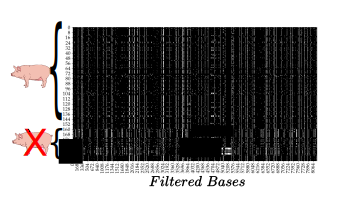
\includegraphics[width=0.85\textwidth]{Sequences.png}
\caption{SNP sequences of Salmonella enterica samples used in this work.
The x-axis shows the genome bases and the y-axis the corresponding sample (210 samples in total).
The black dots are related to a base without mutation (in relation to the genome reference), while the with dots are the mutation (SNPs) identified.
The first 159 rows contains the genome sequences related to pigs, i.e the sequences obtained by a pig which host the bacteria, and the following ones contains sequences of other animals.
Also with naked eyes we can see the differences between the two data types.
}
\label{fig:SNPsAle}
\end{figure}

First of all, we filtered our data removing from each genome a base if it was not mutated in each sample.
In this way we reduced the number of bases to $8189\,bp$.
A graphical representation of these samples is given in Fig.~\ref{fig:SNPsAle}.
The dataset was divided in training and test sets using a stratified cross-validation procedure to guarantee a proportional subdivision of the samples into the two classes.
The algorithm hyper-parameters were tuned on the training set in relation to the performances obtained using a internal stratified 10-fold cross-validation: in each fold the training was performed using a sequence of hyper-parameters and the performances evaluated on the corresponding test set; the hyper-parameters configuration which obtained the best performances on the full training set was chosen as best one.
We use our custom \emph{Score} library for the performance evaluation.
Considering the unbalanced sample quantities the Matthews Correlation Coefficient (MCC) was chosen as good score indicator for the evaluation.

\end{document}

\documentclass{standalone}

\begin{document}


\section[Conclusion]{Conclusion}\label{snp_conclusion}



\end{document}


\documentclass{standalone}

\begin{document}

\section[Byron]{Build YouR Own Neural network - Byron library}\label{byron}

Limits of the most common neural network frameworks.
Neural Network library for parallel computing developed in C++.
Pyron as python wrap of the library.
Description of the algorithms used to optimize the computation (ex. im2col vs winograd).


\end{document}


\documentclass{standalone}

\begin{document}

\section[Yolo]{Object Detection - Yolo architecture}\label{yolo}

%Introduction on the image classification and detection with Yolo architecture.
%Implementation in Byron with description of performances against darknet (original implementation).
%Focus on performances (time, memory, cpu).


\end{document}


\documentclass{standalone}

\begin{document}

\section[Super Resolution]{Super Resolution}\label{SR:sr}

\begin{figure}[htbp]
\def\svgwidth{0.5\textwidth}
\input{./img/sr_wow.pdf_tex}
\quad
\def\svgwidth{0.5\textwidth}
\input{./img/sr_wow2.pdf_tex}
\caption{Single Image Super Resolution.
Between the red lines the super resolved version of the image.
}
\label{fig:sr_wow}
\end{figure}

The Super Resolution (SR) is a slight novel technique based on Neural Network models which aims to improve the spatial resolution of a given image\footnote{
  The best-known \quotes{implementation} of Super Resolution concerns the microscopy super-resolution.
  In this work we are focusing on algorithms and numerical implementation so we will talk about the numerical counterpart of this technique, totally ignoring the original \quotes{hardware} version.
}.

The first SR methods on digital images estimate the high frequency information of the images starting from a series of low-resolution (LR) patches and their high-resolution (HR) counterpart.
These patches (ROIs of the LR image commonly smaller than $50\times50$) were extracted after an edge enhancement procedure or a simple 2D Fourier transform which extract the high frequency information.
Collecting these patches an \quotes{association dictionary} between LR and HR was created.
This dictionary was so used to learn the correct association between the LR e HR counterpart and then applied on new images.
The considered images could also be of the same dimensions in these firstly applications, i.e the purpose was only to improve the spatial resolution of the image without changing the sampling step.

The idea of use neural network models and in particular convolution functions to face on this problem was born in 2014 at the Engineering University of Honk Kong due to the large popularity of these models during that years.
The increasing computational power allowed to create automatic models able to learn the LR-HR association without any dictionary.
In this year arise the SRCNN model~\cite{SRCNN}, a three-layer neural network able to learn a large ensemble of features to reproduce the desired association.
The first layer aimed to extract the LR patches from the input image; the second layer produce the association between the LR patches and the tuned HR ones; the last layer reorganized the HR patches ensemble produced into a single HR image, i.e the output.

From this starting implementation many improvements was performed in this research field but the fundamental idea is not changed.
Modern models simply have a greater number of layers, due to the increasing computational power availability, and they used appropriate workaround to overcome the (large-)parameters tuning problem.

In the next sections we will show the super resolution technique step-by-step starting from the image pre-processing until the most modern algorithmic solutions.
At the end of this chapter the \textsf{NumPyNet} and \textsf{Byron} implementation of some modern models will be presented and applied over biomedical images.

%Introduction on Super Resolution problem with focus on state-of-art neural network architecture.
%Description of the Byron implementation and application on NMR data with the most common measurements.
%Super-resolution allows better detection!


\end{document}


\documentclass{standalone}

\begin{document}

\section[Segmentation]{Image Segmentation}\label{segmentation:unet}

\begin{center}
\begin{figure}[htbp]
\centering
\includegraphics[width=0.85\textwidth]{segmentation.jpg}
\label{fig:segmentation}
\end{figure}
\end{center}

In the previous section we have discussed about the object classification and object detection problems (ref.~\ref{obj_detection:obj}).
Now we want to go deeper on this topic and extract the exact pixels which belong to an object into a given image.
This kind of problem is called Image Segmentation, i.e give a label to each pixel of the input image.

Image segmentation is a typical task in many research fields and could be used for different purposes.
information about pixel-wise position of objects inside an image could be used for extract object shapes from the image or to simplify and/or change the representation of an image into something more meaningful and easier to understand.
This is an hot topic especially for self-driving car applications in which we have to find the exact shapes of object to better estimate their perspective position.
Moreover, all these applications require fast algorithm as much as possible closed to real-time.

This kind of task can be performed using a pipeline of image processing functions or by training a neural network model.
In the first case we have to stack a series of function to process the input image: it has to filters and extracts the useful information about the searched object but most of all it has to be as most general as possible to face on the common heterogeneity of samples.
In the second case we leave to the neural network model parameters the searching of optimal combination of function but we have to provide a supervised input pattern, i.e a combination of input and annotated pixel-wise mask of each image.
The image annotation is one of the most hardest and boring step of image segmentation and for these reasons is very hard to find public dataset usable.

In this chapter we introduce a particular neural network model commonly used in image segmentation problems and we will describe its characteristics and performances.
We applied this model to a novel dataset of CT images.
The dataset annotation was performed by a custom semi-supervised pipeline of image processing and the neural network model was trained and tested on this dataset.
The original data are taken from \href{https://mrl.sci.utah.edu/software/normal-hip-image-data/}{here}~\cite{doi:10.1002/jor.22040} and the corresponding annotations are released on \href{}{here}. % TODO: add google-drive link

\end{document}



\end{document}
